\documentclass[UTF8]{ctexart}
\usepackage{amsmath}
\usepackage{amssymb}
\usepackage{background}
\usepackage{booktabs}
\usepackage{caption,subcaption}
\usepackage{enumitem}
\usepackage{float}
\usepackage{fontspec}
\usepackage{geometry}
\usepackage{makecell}
\usepackage{mathptmx} %mathptmx和times结合使得公式使用times new roman字体
\usepackage{pifont}
\usepackage{tcolorbox}
\tcbuselibrary{breakable, raster}
\usepackage{tikz}
\usetikzlibrary{arrows.meta}
\usepackage{times}
\usepackage{ulem}
\usepackage[table]{xcolor}


\geometry{a5paper, top=0.1cm, left=1cm, right=1cm, bottom=1cm, footskip=0.6cm, marginparsep=0.1cm}

\setCJKmainfont[BoldFont={汉仪文黑-85W},ItalicFont={方正苏新诗柳楷简体}]{汉仪文黑-55W}
\setfontfamily\Issue{Century Schoolbook}
\setfontfamily\Genshin{Genshin Teyvat Lingua Franca}
\newfontfamily\timesnewroman{Times New Roman}
\setmainfont{Times New Roman}
\newCJKfontfamily\TitleFont{思源宋体 CN Heavy}
\captionsetup{font=small, labelfont=bf}
\setlist[itemize]{itemsep=0pt, parsep=0pt}
%\reversemarginpar

%\CTEXsetup[format = {\centering\bfseries\large}, beforeskip = 3pt, afterskip = 3pt]{section}
\CTEXsetup[format = {\color{cyan!50!black}\bfseries\large}]{subsection}

\newtcolorbox{mybox}{colback=cyan!10, colframe=cyan!50!black, boxrule=0.5pt, breakable}

\colorlet{color1}{blue}
\colorlet{color1b}{blue!20!white}
\colorlet{color2}{green!50!black}
\colorlet{color2b}{green!20!white}
\colorlet{color3}{violet}
\colorlet{color3b}{violet!20!white}

\colorlet{darkcyan}{cyan!50!black}
\newcommand\Black[1]{\textcolor[gray]{0.3}{#1}}
\newcommand\Brown[1]{\textcolor[HTML]{998A4E}{#1}}
\newcommand\Emph[1]{\colorbox{green!10}{\textcolor{green!30!black}{#1}}}
\newcommand\Concept[1]{\textcolor{cyan!70!black}{#1}}
\newcommand\Notes[1]{\textcolor{yellow!50!black}{\small #1}}
\newcommand\Example[1]{\textcolor{cyan!70!black}{\small #1}}
\newcommand\means[1]{\textcolor{cyan!70!black}{#1}}

\renewcommand\O{\mathrm{O}}

\newcommand\IssueNumber{29}
\newcommand\Date{2024-6-1}
%\newcommand\Contributer{@金光日}
\newcommand\Subject{数据结构与算法}
%\newcommand\Source{2022 考研 408 第 5 题}


\begin{document}
\backgroundsetup{contents=
\includegraphics{上半示例.png}, center, scale=1, angle=0, opacity=1}
\BgThispage
\begin{center}
%{\scriptsize\Issue \textcolor[HTML]{C8BA83}{\Genshin WEEKLY TIPS}}
\phantom{...}

{\Large\textcolor{brown!40!white}{\makebox[10cm][s]{\Genshin WEEKLY KNOWLEDGE TIPS}}}

\vspace{-2em}

{\Huge\bfseries\TitleFont \Black{知\ 识\ 小\ 料}}


\vspace{-0.1cm}
{\footnotesize \Brown{「电计 2203 班」周常规知识整理共享}}
\end{center}

\vspace{-0.5cm}


\begin{figure}[H]
\hspace{1cm}
\begin{minipage}[t]{0.3\textwidth}
\centering
    \Brown{\Genshin ISSUE}

    \vspace{-0.6cm}
    \Huge \Issue\slshape\bfseries\Black{\IssueNumber}
\end{minipage}
\hfill
\begin{minipage}[t]{0.35\textwidth}
\small
\centering
    \Brown{日期:\Date} \\
%\vspace{-0.1cm}
%    \Brown{贡献者:\Contributer} \\
\vspace{-0.1cm}
    \Brown{学科:\Subject} \\
%\vspace{-0.1cm}
%    \Brown{来源:\Source}
\end{minipage}
\hspace{0.8cm}
\end{figure}

\begin{center}
\textcolor{cyan!50!black}{常用排序算法简易总结}
\end{center}

\newcommand\correct{\textcolor{green!50!black}{\ding{51}}}
\newcommand\wrong{\textcolor{red!70!black}{\ding{55}}}
\begin{table}[htb]
  \centering
  \begin{tabular}{cccccc}
\toprule
    \textbf{排序算法} & \textbf{平均时间} & \textbf{最好} & \textbf{最坏} & \textbf{空间} & \textbf{是否稳定} \\
\midrule
    冒泡排序 & $\O(n^2)$ & $\O(n)$ & — & $\O(1)$ & \correct \\
    插入排序 & $\O(n^2)$ & $\O(n)$ & — & $\O(1)$ & \correct \\
    选择排序 & $\O(n^2)$ & — & — & $\O(1)$ & \wrong \\
    快速排序 & $\O(n\log n)$ & — & $\O(n^2)$ & $\O(\log n)$ & \wrong \\
    堆排序 & $\O(n\log n)$ & — & — & $\O(1)$ & \wrong \\
    归并排序 & $\O(n\log n)$ & — & — & $\O(n)$ & \correct \\
    希尔排序 & $\O(n^{1.5})$ & $\O(n)$ & $\O(n^2)$ & $\O(1)$ & \wrong \\
    计数排序 & $\O(n+k)$ & — & — & $\O(k)$ & \correct \\
    基数排序 & $\O(d\cdot(n+2r))$ & — & — & $\O(r)$ & \correct \\
\bottomrule
\end{tabular}
  \caption{常用排序算法总表(横线表示与平均时间复杂度一致)}\label{tab:total}
\end{table}

%%% 定义排序好的元素
\newcommand\sort[1]{\colorbox{color1b}{\textcolor{color1}{#1}}}

\paragraph{\textcolor{color1}{冒泡排序}} {\small\textcolor{color1}{($\O(n^2)$ · 稳定)}}

在每轮中使一个数与其后一个数交换,将最大值排到右侧,使右侧有序。

\begin{table}[H]
  \centering
  \begin{tabular}{ccccccccc}
    初始 & 50 & 86 & 72 & 41 & 45 & 93 & 57 & 46 \\
    一次 & 50 & 72 & 41 & 45 & 86 & 57 & 46 & \sort{93} \\
    二次 & 50 & 41 & 45 & 72 & 57 & 46 & \sort{86} & \sort{93} \\
  \end{tabular}
\end{table}

\vspace{-2em}

\paragraph{\textcolor{color1}{插入排序}} {\small\textcolor{color1}{($\O(n^2)$ · 稳定)}}

在每轮中将待排序元素插入到序列左侧的恰当位置,使左侧有序。

\begin{table}[H]
  \centering
  \begin{tabular}{ccccccccc}
    初始 & \sort{50} & 86 & 72 & 41 & 45 & 93 & 57 & 46 \\
    一次 & \sort{50} & \sort{86} & 72 & 41 & 45 & 93 & 57 & 46  \\
    二次 & \sort{50} & \sort{72} & \sort{86} & 41 & 45 & 93 & 57 & 46 \\
  \end{tabular}
\end{table}

\newpage
\backgroundsetup{contents=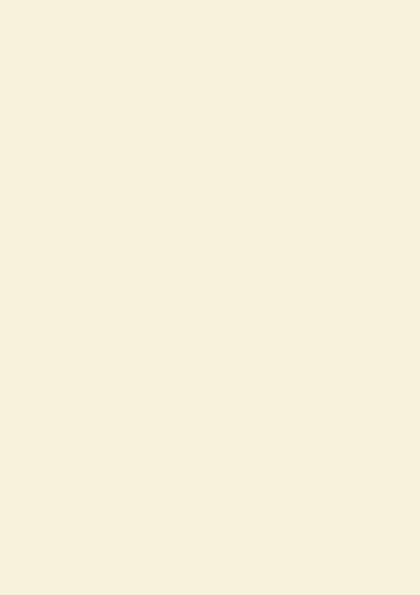
\includegraphics{空白示例.png}, center, scale=1, angle=0, opacity=1}
\BgThispage

\paragraph{\textcolor{color1}{选择排序}} {\small\textcolor{color1}{($\O(n^2)$ · 不稳定)}}

在每轮中找一个最小值,与乱序序列中的第一个数交换,使左侧有序。

\begin{table}[H]
  \centering
  \begin{tabular}{ccccccccc}
    初始 & 50 & 86 & 72 & \uline{41} & 45 & 93 & 57 & 46 \\
    一次 & \sort{41} & 86 & 72 & 50 & \uline{45} & 93 & 57 & 46 \\
    二次 & \sort{41} & \sort{45} & 72 & 50 & 86 & 93 & 57 & 46 \\
  \end{tabular}
\end{table}


\renewcommand\sort[1]{\colorbox{color2b}{\textcolor{color2}{#1}}}
\paragraph{\textcolor{color2}{快速排序}} {\small\textcolor{color2}{($\O(n\log n)$·不稳定)}}

在每轮中取一个基准,通过双指针,使比基准小的元素都在左侧,比基准大的都在右侧。

\begin{table}[H]
  \centering
  \begin{tabular}{ccccccccc}
    初始 & \uline{50} & 86 & 72 & 41 & 45 & 93 & 57 & 46 \\
    一次 & \uline{46} & 45 & 41 & \sort{50} & \uline{72} & 93 & 57 &  86 \\
    二次 & 41 & 45 & \sort{46} & \sort{50} & 57 & \sort{72} & 93 & 86 \\
  \end{tabular}
\end{table}

\paragraph{\textcolor{color2}{堆排序}} {\small\textcolor{color2}{($\O(n\log n)$·不稳定)}}

在每轮中通过构建大根堆的方式排序。从第 $\frac{n}{2}$ 个数开始,每次调整时维护大根堆性质,并递归地维护其子树,直到根节点(堆顶)。随后将堆顶与最后一个乱序数交换,使右侧有序。(要理解下列例子,请画出对应的堆。)

\begin{table}[H]
  \centering
  \begin{tabular}{ccccccccc}
    初始 & 50 & 86 & 72 & 41 & 45 & 93 & 57 & 46 \\
    一次 & \uline{93} & 86 & 72 & 46 & 45 & 50 & 57 & 41 \\
    交换 & 41 & 86 & 72 & 46 & 45 & 50 & 57 & \sort{93} \\
    二次 & \uline{86} & 46 & 72 & 41 & 45 & 50 & 57 & \sort{93} \\
    交换 & 57 & 46 & 72 & 41 & 45 & 50 & \sort{86} & \sort{93} \\
  \end{tabular}
\end{table}

\paragraph{\textcolor{color2}{归并排序}} {\small\textcolor{color2}{($\O(n\log n)$·稳定)}}

在每轮中通过将区间递\textcolor{color2}{\textbf{归}}地划分为左右两部分,随后将两部分\textcolor{color2}{\textbf{并}}起来排序。

\begin{table}[H]
  \centering
  \begin{tabular}{ccccccccc}
    初始 &[50] & [86] & [72] & [41] & [45] & [93] & [57] & [46] \\
    一次 &[50 & 86] & [41 & 72] & [45 & 93] & [46 & 57] \\
    二次 &[41 & 50 & 72 & 86] & [45 & 46 & 57 & 93] \\
  \end{tabular}
\end{table}

\renewcommand\sort[1]{\colorbox{color3b}{\textcolor{color3}{#1}}}
\paragraph{\textcolor{color3}{希尔排序}} {\small\textcolor{color3}{($\O(n^{1.5})$·不稳定)}}

在每轮中通过间隔分组的方式在组内排序,随轮次增加而缩小间隔。下列的例子中同种颜色的色块为一组,$d_1=4$,$d_2=2$。

\newpage
\backgroundsetup{contents=
\includegraphics{下半示例.png}, center, scale=1, angle=0, opacity=1}
\BgThispage

\begin{table}[H]
  \centering
  \begin{tabular}{ccccccccc}
    初始 & 50 & 86 & 72 & 41 & 45 & 93 & 57 & 46 \\
    一次 & \colorbox{red!20!white}{\textcolor{red!50!black}{45}} &
    \colorbox{blue!20!white}{\textcolor{blue}{86}} &
    \colorbox{green!20!white}{\textcolor{green!50!black}{57}} &
    \colorbox{yellow!20!white}{\textcolor{yellow!50!black}{41}} &
    \colorbox{red!20!white}{\textcolor{red!50!black}{50}} &
    \colorbox{blue!20!white}{\textcolor{blue}{93}} &
    \colorbox{green!20!white}{\textcolor{green!50!black}{72}} &
    \colorbox{yellow!20!white}{\textcolor{yellow!50!black}{46}} \\
    二次 & \colorbox{red!20!white}{\textcolor{red!50!black}{45}} &
    \colorbox{blue!20!white}{\textcolor{blue}{41}} &
    \colorbox{red!20!white}{\textcolor{red!50!black}{50}} &
    \colorbox{blue!20!white}{\textcolor{blue}{46}} &
    \colorbox{red!20!white}{\textcolor{red!50!black}{57}} &
    \colorbox{blue!20!white}{\textcolor{blue}{86}} &
    \colorbox{red!20!white}{\textcolor{red!50!black}{72}} &
    \colorbox{blue!20!white}{\textcolor{blue}{93}} \\
  \end{tabular}
\end{table}

\paragraph{\textcolor{color3}{计数排序}} {\small\textcolor{color3}{($\O(n+k)$·稳定)}}

一种实现方法是,用数组 $\{c_i\}$ 记录元素 $i$ 出现的次数,遍历数组并记录每个元素的出现次数,随后清空 $\{c_i\}$。需要知道数组元素的分布。下例采用本方法。

另一种方法是,用 $\{c_i\}$ 记录比 $i$ 小的数的个数,对每个元素 $a_i$ 应满足 $i=c_i+1$,如果不是则对调 $a_{i}$ 与 $a_{c_i+1}$ 的值,直到所有元素满足。

具体时间复杂度 $\O(n+k)$,$n$ 为元素个数,$k$ 为数据范围(可能的数值个数)。


\begin{table}[H]
  \centering
  初始:3\quad 5\quad 5\quad 2\quad 4

  \begin{tabular}{ccccccccc}
  \toprule
  \rowcolor{violet!20}
  $i$ & 0 & 1 & 2 & 3 & 4 & 5 \\
  \rowcolor{violet!10}
  $c_i$ & 0 & 0 & 1 & 1 & 1 & 2 \\
  \bottomrule
  \end{tabular}

  排序:2\quad 3\quad 4\quad 5\quad 5\\
\end{table}

\paragraph{\textcolor{color3}{基数排序}} {\small\textcolor{color3}{($\O(d\cdot(n+2r))$·稳定)}}

在每轮中分别以某一位为关键字,从个位起,使该位及所有低位均有序。

具体时间复杂度 $\O(d\cdot(n+2r))$,$d$ 为关键字个数(数字位数),$n$ 为数据个数,$r$ 为「基」即关键字取值的个数。

\begin{table}[H]
  \centering
  \begin{tabular}{ccccccccc}
    初始 & 38 & 125 & 474 & 368 & 16 & 30 & 590 & 372 \\
    一轮 & 03\uline{0} & 59\uline{0} & 37\uline{2} & 47\uline{4} & 12\uline{5} & 01\uline{6} & 03\uline{8} & 36\uline{8} \\
    二轮 & 0\uline{16} & 1\uline{25} & 0\uline{30} & 0\uline{38} & 3\uline{68} & 3\uline{72} & 4\uline{74} & 5\uline{90} \\
  \end{tabular}
\end{table}

\paragraph{\textcolor{color3}{不稳定算法分析用例}}
以下例子中 2 位于 $2'$ 的左侧,但排序过后 2 移到 $2'$ 的右侧,也就是相同值的元素的相对位置发生了改变。

\begin{figure}[htb]
\begin{minipage}[b]{.245\textwidth}
    \centering
    选择排序
    \begin{tabular}{cccc}
    \toprule
     & 2 & $2'$ & 1 \\
    I & \sort{1} & $2'$ & 2 \\
    II & \sort{1} & \sort{$2'$} & 2 \\
    III & \sort{1} & \sort{$2'$} & \sort{2} \\
    \bottomrule
    \end{tabular}
\end{minipage}
\begin{minipage}[b]{.245\textwidth}
    \centering
    快速排序
    \begin{tabular}{cccc}
    \toprule
     & 2 & $2'$ & 1\\
    I & 1 & $2'$ & \sort{2} \\
    II & \sort{1} & $2'$ & \sort{2} \\
    III & \sort{1} & \sort{$2'$} & \sort{2} \\
    \bottomrule
    \end{tabular}
\end{minipage}
\begin{minipage}[b]{.245\textwidth}
    \centering
    堆排序
    \begin{tabular}{cccc}
    \toprule
     & 2 & $2'$ & 1\\
    I & 1 & $2'$ & \sort{2} \\
    II & 1 & \sort{$2'$} & \sort{2} \\
    III & \sort{1} & \sort{$2'$} & \sort{2} \\
    \bottomrule
    \end{tabular}
\end{minipage}
\begin{minipage}[b]{.245\textwidth}
    \centering
    希尔排序
    \begin{tabular}{cccc}
    \toprule
     & 2 & $2'$ & 1\\
    I & \colorbox{red!20!white}{\textcolor{red!50!black}{1}} & \colorbox{blue!20!white}{\textcolor{blue}{$2'$}} &
    \colorbox{red!20!white}{\textcolor{red!50!black}{2}} \\
    II & \colorbox{red!20!white}{\textcolor{red!50!black}{1}} & \colorbox{red!20!white}{\textcolor{red!50!black}{$2'$}} & \colorbox{red!20!white}{\textcolor{red!50!black}{2}} \\
    \multicolumn{4}{c}{$(d_1=2, d_2=1)$} \\
    \bottomrule
    \end{tabular}
\end{minipage}
\end{figure}

\end{document} 